\documentclass[10pt, conference, compsocconf]{IEEEtran}

% Various packages that might be useful
\usepackage[pdftex]{graphicx}
\usepackage{array}
%\usepackage[tight,footnotesize]{subfigure}
%\usepackage{url}
\hyphenation{op-tical net-works semi-conduc-tor}
\usepackage{color}
\usepackage{underscore}


\begin{document}

\title{Production Experiences with the Cray-Enabled TORQUE Resource Manager}

\author{\IEEEauthorblockN{Matt Ezell and Don Maxwell}
\IEEEauthorblockA{High Performance Computing Operations\\
Oak Ridge National Laboratory\\
Oak Ridge, TN\\
\{ezellma,maxwellde\}@ornl.gov}
\and
\IEEEauthorblockN{David Beer}
\IEEEauthorblockA{Senior Software Engineer\\
Adaptive Computing\\
Provo, UT\\
dbeer@adaptivecomputing.com}
}

\maketitle


\begin{abstract}
High performance computing resources utilize batch systems to manage the user
workload. Cray systems are uniquely different from typical clusters due to
Cray’s Application Level Placement Scheduler (ALPS). ALPS manages binary
transfer, job launch and monitoring, and error handling. Batch systems require
special support to integrate with ALPS using an XML protocol called BASIL.

Previous versions of Adaptive Computing’s TORQUE and Moab batch suite integrated
with ALPS from within Moab, using PERL scripts to interface with BASIL. This
would occasionally lead to problems when all the components would become
unsynchronized. Version 4.1 of the TORQUE Resource Manager introduced new
features that allow it to directly integrate with ALPS using BASIL. This paper
describes production experiences at Oak Ridge National Lab using the new TORQUE
software versions.
\end{abstract}

\begin{IEEEkeywords}
TORQUE; Resource Manager; Adaptive Computing; Cray; ALPS; Moab; HPC; Titan; Gaea
\end{IEEEkeywords}


\section{Introduction}

High performance computing resources utilize batch systems to manage the user
workload. Job schedulers are designed to intelligently determine when jobs
should run, optimizing for various goals such as high utilization or minimal
queue wait. Resource managers typically accept job submissions and handle job
launch. Cray systems are uniquely different from typical clusters due to an
additional layer called Cray's Application Level Placement Scheduler (ALPS).
ALPS manages binary transfer, job launch and monitoring, and error handling.
Batch systems require special support to integrate with ALPS using an XML
protocol called BASIL.

Previous versions of Adaptive Computing's TORQUE and Moab batch suite
integrated with ALPS from within Moab, using PERL scripts to interface with
BASIL. This would occasionally lead to problems when all the components would
become unsynchronized. Additionally, TORQUE was unaware of the Cray compute
nodes. Version 4.1 of the TORQUE Resource Manager introduced new features that
allow it to directly integrate with ALPS using the BASIL protocol.

This paper describes early experiences with the newest versions of the TORQUE
resource manager. Early on, software bugs related to the newly-introduced
multithreading features prevented successful deployment of the new versions of
TORQUE. Through close collaboration with Adaptive Computing, the software
improved significantly to the point where it was acceptable for use on the
Titan and Gaea systems. Additionally, this paper describes production
experiences at Oak Ridge National Laboratory using the new TORQUE software
versions and describes future collaborative work to improve Cray-enabled
TORQUE.


\section{Cray Application Level Placement Scheduler (ALPS)}

\begin{figure*}
  \centering
  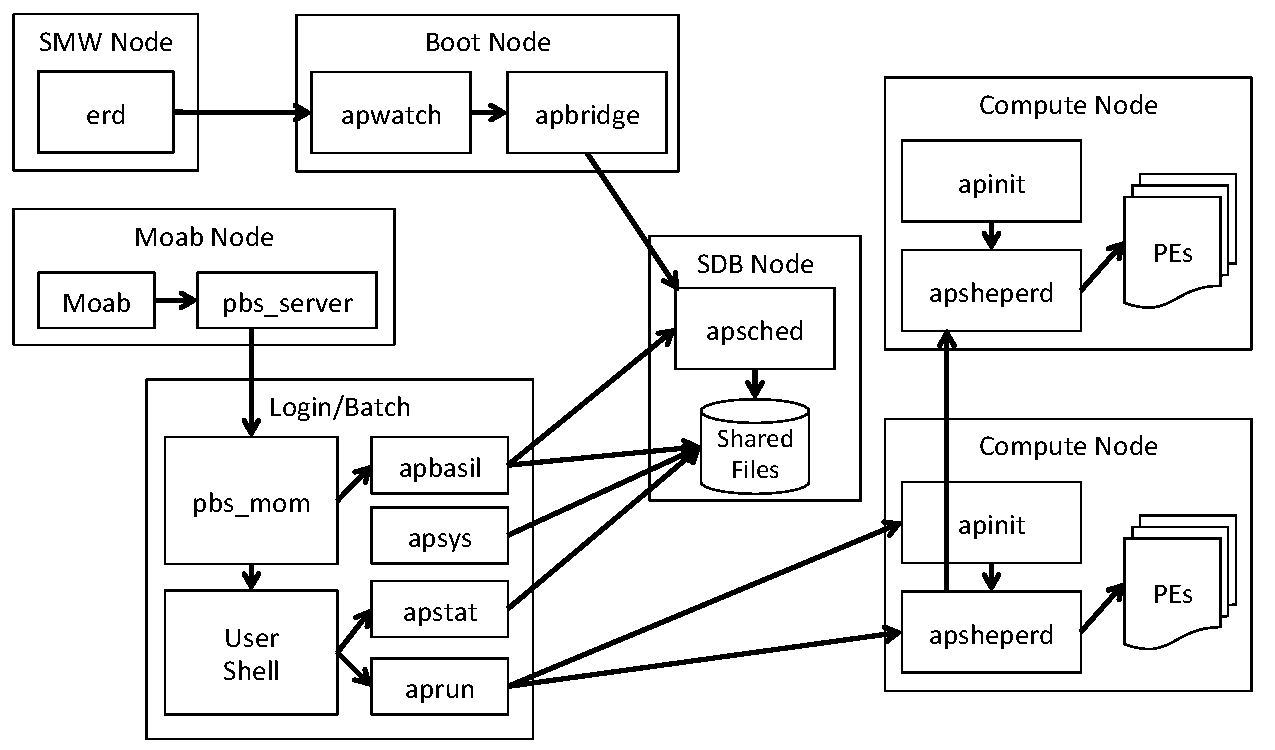
\includegraphics[width=6.5in]{figures/alps-hilevel.pdf}\\
  \caption{High-Level ALPS Design}\label{fig:alps-hilevel}
\end{figure*}

The term ``resource manager'' is overloaded in the batch processing world, and
the combination of systems needed to effectively control batch processing on
the Cray X-series platform certainly supports the confusion.  At the lowest
level in the Cray hierarchy sits the Cray Application Level Placement Scheduler,
commonly referred to as ALPS \cite{alps}.  While in most instances, a batch
system is making scheduling decisions based upon configuration of center
policy, ALPS is the piece of software at the lowest level that is handed
information from the batch system to ultimately launch the job onto the compute
nodes.

Not only does ALPS launch jobs, it maintains compute node state and
reservations to manage job placement and resource utilization.  Through a
series of daemons that typically run on the Cray boot or system database (sdb)
node, ALPS imports hardware configuration information from the system database
to provide memory, CPU and GPU resources available on each compute node.  Given
a heterogeneous system, this would be essential to providing the user with a
mechanism to request the resources needed to run a particular application.
Each compute node also has a state and mode associated with it that informs
ALPS whether the node is up or down and whether it is in interactive or batch
mode.  Up and down states are self-explanatory, and there are a few other
states that will not be discussed that are in the end classified as up or down,
but interactive or batch mode requires some explanation.  

ALPS can operate without a batch system sitting at a higher level providing
information.  This is called interactive mode, and it is basically a FIFO queue
that requires users to run ALPS commands that sit and wait for available
resources to run jobs.  How is this different from a batch system?  In a
nutshell, batch systems provide a mechanism for the user to submit a job to be
run at a later time without the burden of making sure the machine doesn't
reboot taking the waiting ALPS command down with it. Batch systems also allow a
priority-based reordering of jobs based on policies determined by the center.
In contrast, batch mode simply enables the use of a batch system for job launch
ignoring any user-supplied ALPS commands run outside of the batch system.

Reservations are used to manage availability of nodes that are in an up state.
When a job is launched, it is assigned to a set of nodes. Those nodes are
exclusively reserved for that job.  When the job finishes, the reservation is
destroyed, and those nodes are available for the next job.  Reservations are
simply the mechanism by which a job receives exclusive access to the resources
necessary to run the job.

All of the ALPS information must somehow get communicated to the batch system
in order to provide the user with the available resources on the system and to
maintain a consistent state for nodes, reservations, and jobs.  ALPS provides
an API called \emph{apbasil} - BASIL being an acronym for Batch Application
Scheduler Interface Layer.  BASIL is an XML-based protocol that provides batch
systems with the ability to retrieve inventories of compute nodes, their states
and reservations, and the ability to create, confirm, and delete reservations.
Using this interface, batch systems are able to manage all aspects of job
submission, scheduling, placement and deletion by communicating with ALPS which
communicates directly with the compute nodes.


\section{Moab-ALPS Integration Design}

Prior to TORQUE version 4.1, the primary interaction between the batch system
and ALPS was managed by Moab.  Moab has the concept of a ``native'' interface
that allows external scripts to handle logic in user-configurable ways.  For
Cray systems, the TORQUE resource manager was setup as a native interface.
Multiple scripts were provided to manage reservation creation and deletion as
well as job launch:

\begin{description}
  \item[node.query.xt4.pl] \hfill \\
    This script queries BASIL to get the configuration and state of all compute nodes on the system
  \item[job.query.xt4.pl] \hfill \\
    The job query script executes and parses TORQUE commands to obtain a list of all jobs known to the system, including details such as state, owner, account, queue, and resource requests.
  \item[job.start.xt4.pl] \hfill \\
    This script determines the best pbs_mom to host the job and forces execution on this node
  \item[partition.query.xt4.pl] \hfill \\
    The partition query script talks to both ALPS and TORQUE to determine what ALPS reservations exist and if they correspond to a running job
  \item[partition.create.xt4.pl] \hfill \\
    This script interfaces with BASIL to create a reservation based on the resource requests of a job. It does not confirm the request, as this must be done by TORQUE once the SID or PAGG is known
  \item[partition.delete.xt4.pl] \hfill \\
    The partition delete script, as its name implies, is used to remove ALPS reservations once jobs have completed
\end{description}


\section{New Design}

\subsection{Orphan ALPS Reservations}

The new design greatly simplifies the implementation by reducing integration points and
coupling things where they naturally make sense. The minutiae of creating, confirming, and
releasing jobs doesn't need to be performed by a scheduler; moving this all to mom daemons
allows Moab to do what it does best – schedule. Mom daemons already manage everything that 
has to do with setting up jobs, starting them, and cleaning up after them once completed, 
so the ALPS interactions belong on the moms. Finally, having all of the integration a 
single daemon reduces integration points, making the code easier to understand and maintain.

\subsection{How It Works}
\begin{figure}
  \centering
  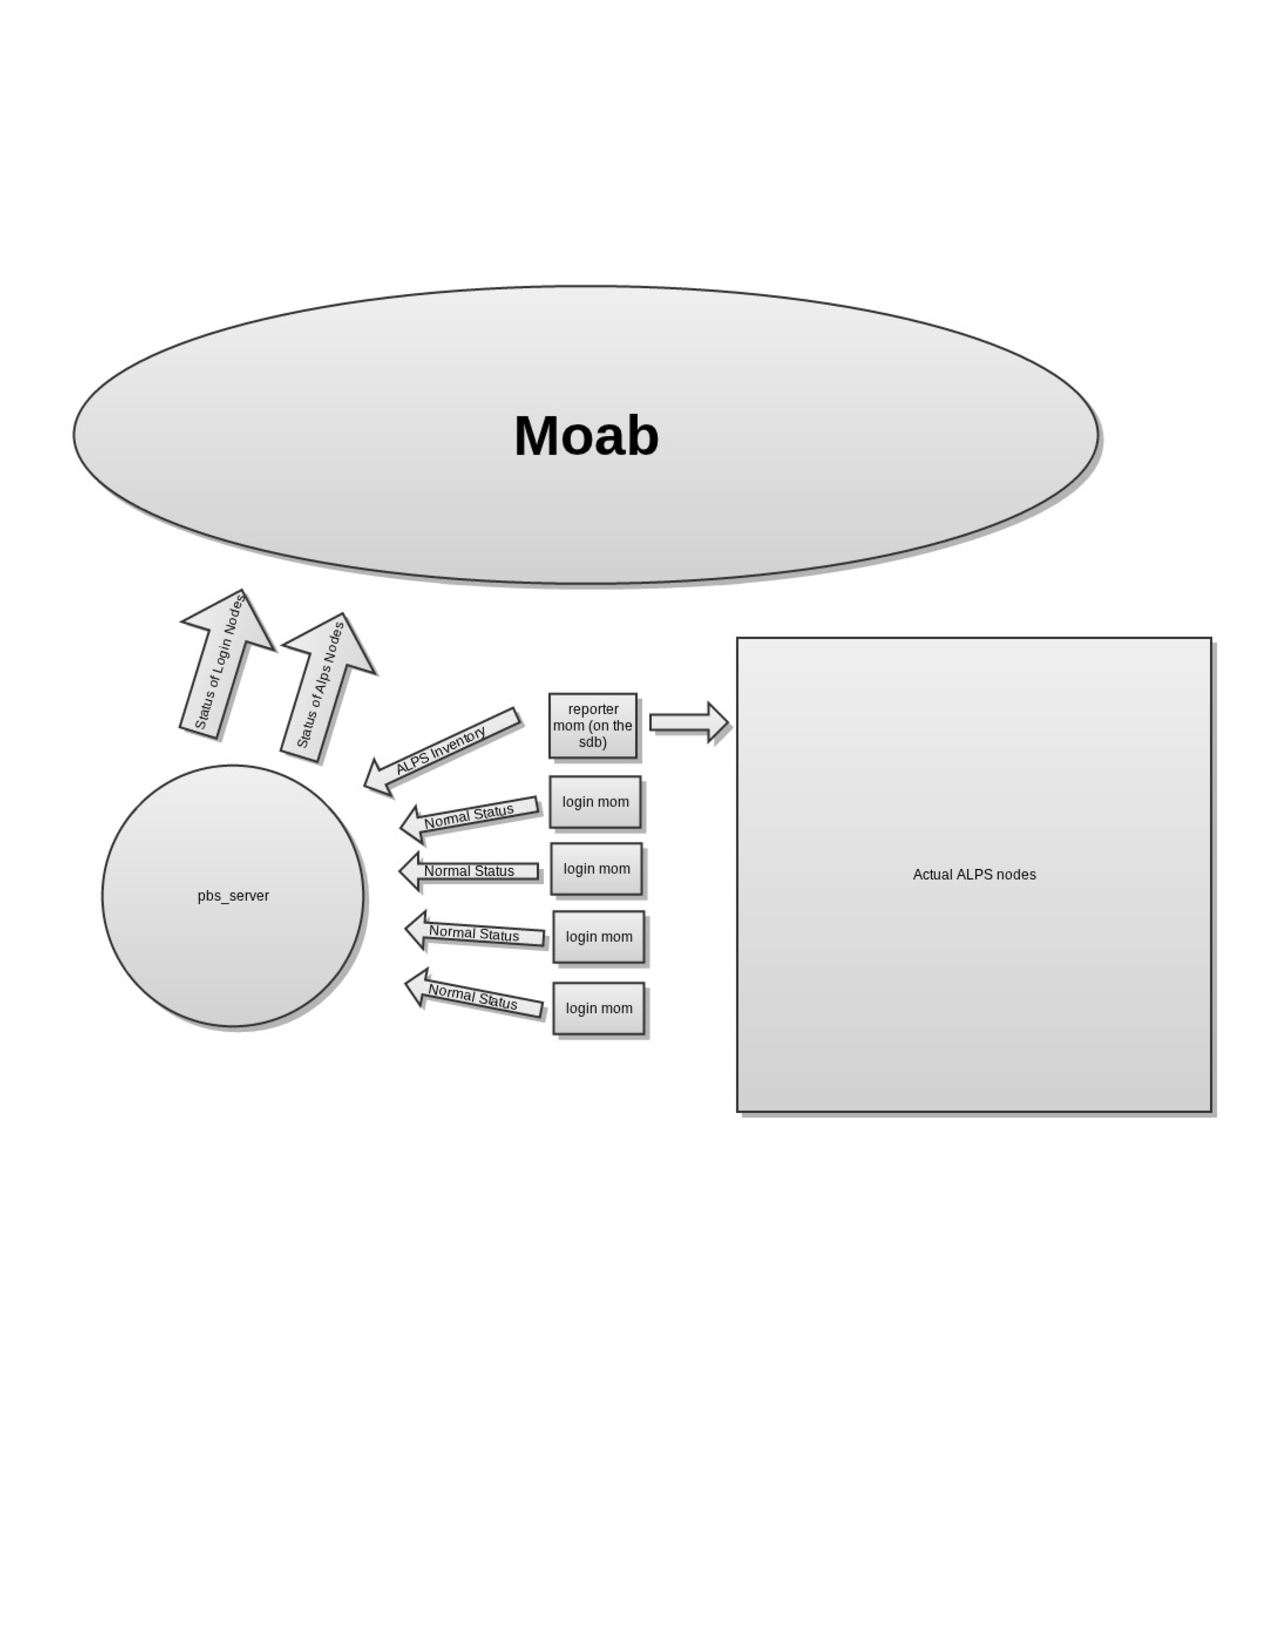
\includegraphics[width=5.0in]{figures/new_diagram.pdf}
  \caption{New Reporting Structure}\label{fig:reporting}
\end{figure}

All ALPS integration now takes place on the mom daemons. Two different kinds of mom daemons are
run for this setup: a reporter mom and one or more alps_login moms. The reporter mom's only function is to report
the inventory information to pbs_server, which then discovers all of the computes. 

The other mom daemon is the alps_login type, which manages job starts. The login mom creates and confirms
the reservations for the job before launching it. When the job is done, the mom releases its ALPS
reservation. The job start process is diagramed below in \ref{fig:starting}.

Moab no longer knows anything about ALPS. From Moab's perspective, it is scheduling a two different
partitions (clusters) - the login nodes in one partition and the compute nodes in the other. Moab is
only making scheduling decisions, and so it is now only given information relevant to scheduling. This is 
outlined in \ref{fig:reporting}. Moab maintains the ability to schedule login-only jobs for the 
purpose of compilation or other simple, short tasks. 

The pbs_server ties the two together. When a node status is given, the reporter mom's status is presented
as the status of all of the compute nodes, and the logins' statuses are given as any other pbs_mom's 
status appears. When Moab runs a job, it only selects which compute nodes that job will use, and pbs_server
uses a round robin method to select which login daemon should be responsible for starting that job. 

\begin{figure}
  \centering
  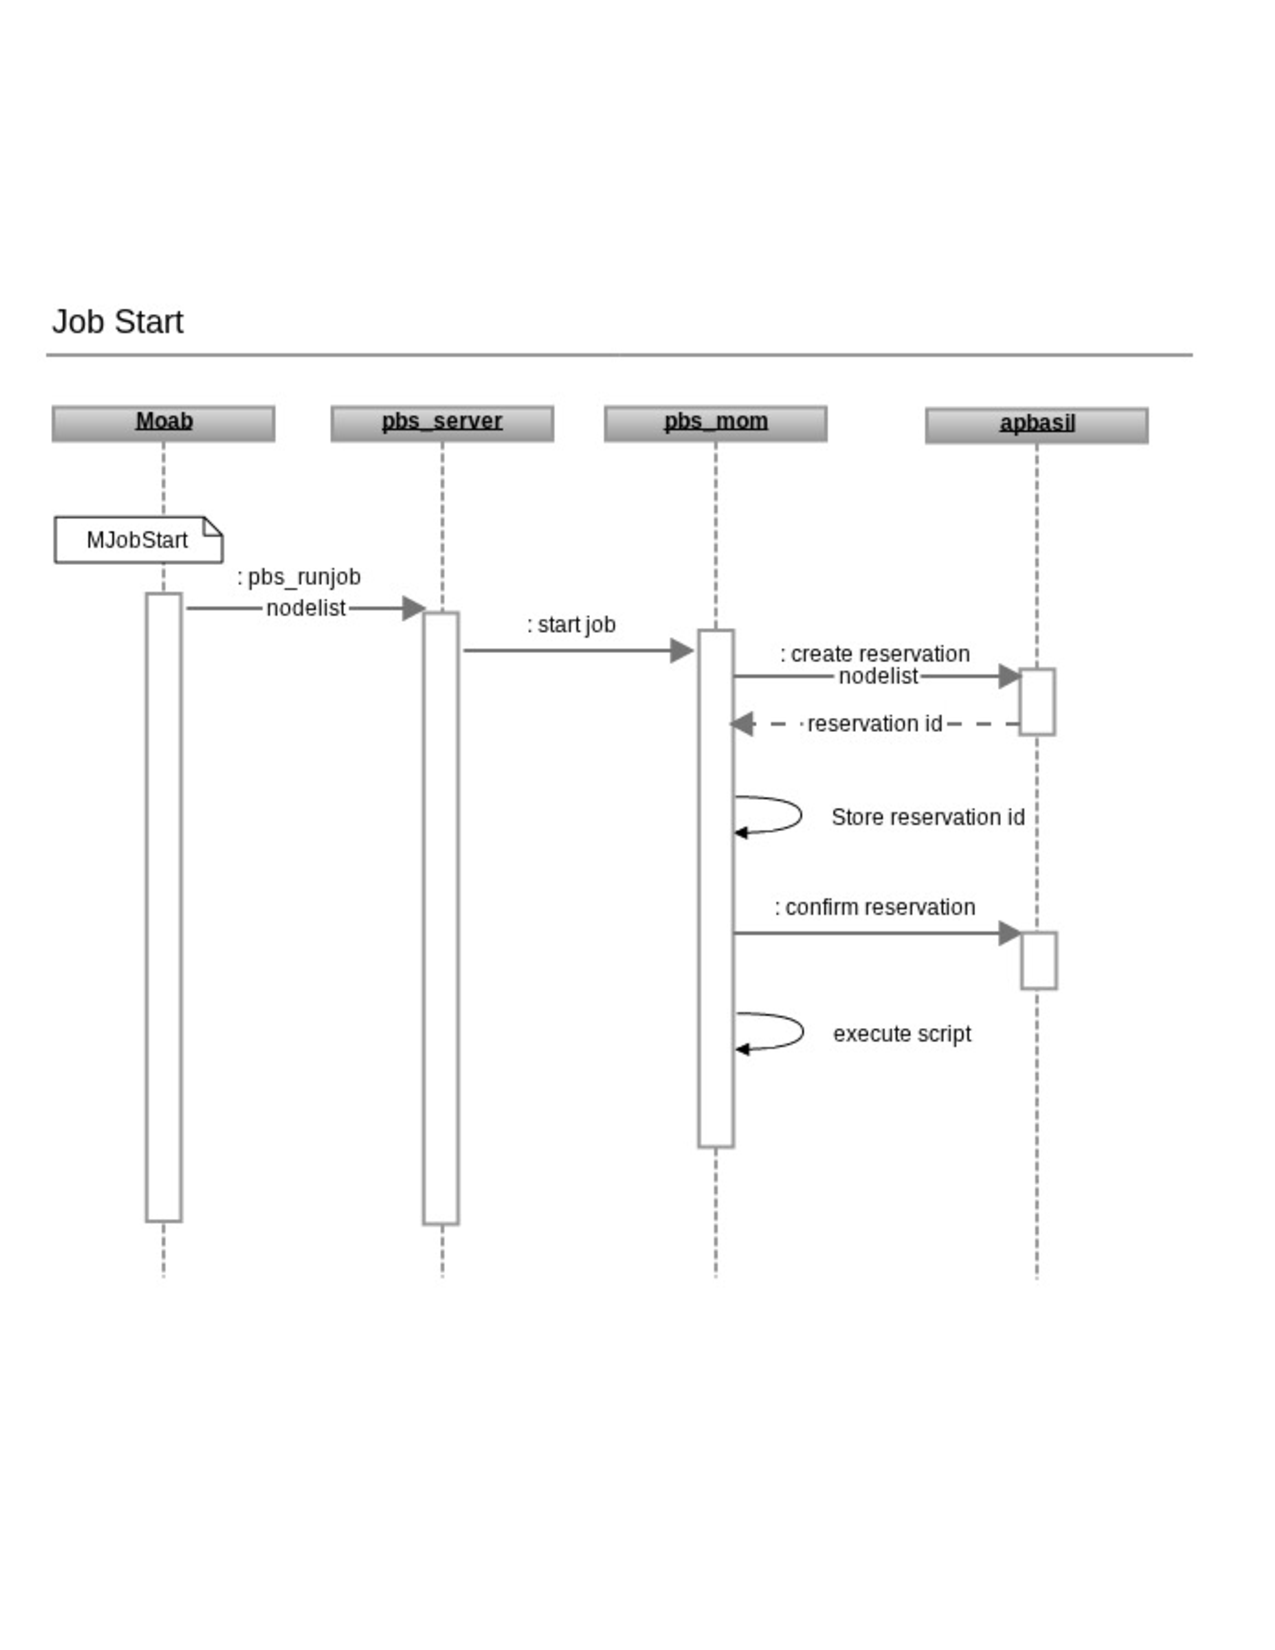
\includegraphics[width=3.0in]{figures/job_start.pdf}
  \caption{Job Starting}\label{fig:starting}
\end{figure}

\subsection{Advantages}
The new design simplifies configuration. No special binaries for Moab, TORQUE's server or mom
daemons are required, not even for the distinct types of mom daemons. Less configuration makes
for easier setup.

The whole model inherits superior support from Moab because from Moab's perspective, scheduling 
the Cray is the same as scheduling any other cluster, and it is no longer a one-off. Additionally,
the code path that was used for parsing output from the scripts in significantly slower than the 
code path for interfacing with TORQUE for two reasons: text parsing happens faster and the interaction
is now through an API instead of a fork/pipe model.

Moab and pbs_server can now be moved outside of the Cray, allowing a number of benefits. You can
install them on as powerful of nodes as you like, and aren't bound to whatever you have already.
If, after having the machine for a while, you decide you need to upgrade the server and scheduler
nodes then you can do this without upgrading the entire machine. This also gives you back whatever
resources on the Cray Moab and pbs_server were occupying. 

\section{Production Experiences}

\subsection{Experiences on Gaea}


\subsection{Experiences on Titan}

While Jaguar never ran the new architecture aside from the beta test shot,
Titan began its life in September 2012 running the new design.  While many of
the issues inherent in a new design had already been discovered and fixed
during both the beta and subsequent use on the TDS’s, the Titan acceptance team
put the new software stack through its paces at scale for true production.
This transition also provided a new opportunity to externalize both Moab and
TORQUE servers from the Cray platform to provide job access for users even when
the Cray was unavailable.  Two fundamental changes at once is generally not a
good idea, but all in all, things have gone fairly well.

Overwhelmingly, the primary problem that has been seen on Titan is deadlocks in
the TORQUE server.  Threading the version 4 TORQUE server is clearly a step in
the right direction, but it has come with some growing pains.  A deadlocked
TORQUE server causes issues for the entire batch system from simple job
submission failure to a hung or at least very slow Moab server.  Primarily due
to the fact that the end users were seeing job submission failures, a script
was created early in the acceptance period which first determined the TORQUE
server was deadlocked, gdb attached to the server and generated a core file,
and then restarted the server.  By running this script on a regular schedule
via cron, the pain felt by the users became much more bearable until the
deadlocks were found and fixed.  Through the efforts of both ORNL and Adaptive
staff, all known deadlocks have been fixed, and the batch system is running
well at this point. 

The transition to an external Moab and TORQUE server has certainly been well
received by the users.  Having the ability to manipulate jobs when the Cray is
unavailable provides the user with everything needed for the job process except
the actual execution.  Some effort had to be devoted to finding a TORQUE server
bug that prevented this from working, but that has now been fixed as well.

Again, the transition to the new architecture and the external servers has been
a success in spite of a few growing pains.  Ultimately, the users have seen
benefits from both better synchronization with ALPS and the ability to
manipulate jobs while the Cray itself is unavailable.



\section{Future Work}


\section{Conclusion}


\section*{Acknowledgment}

The authors would like to thank the TORQUE developers as well as the TORQUE
community for constantly improving TORQUE.


% references section
\bibliographystyle{IEEEtran}
\bibliography{IEEEabrv,cug2013-torque}

% that's all folks
\end{document}


